\chapter{Background}
\label{chap:background}
In this chapter, we will provide the basic knowledge of the techniques used in this project, including the RNN, the branch prediction, the dataset, and the methods used during training. We will first present the basic concept of each technique, and then the relevant literature will be provided.

\section{Recurrent Neural Network}
\label{sec:rnn}
\subsection{Basic Knowledge}
\label{sec:bk_rnn}
RNN is a type of neural network, different from the feed-forward neural network, RNN could remember the information from the previous input data, which benefits from the recurrent pattern inside the RNN units. Figure ~\ref{fig:unrolled} shows the structure of the vanilla RNN and the unrolling version. We could see that the output $o_t$ depends on both the input at time $t$ ($x_t$) and the previous hidden state $s_{t-1}$. The output at time $t$ could be calculated by the euations below, where $f$ could be a nonlinear function.

\begin{equation}
\begin{aligned}
s_t = f(Ux_t + Ws_{t-1})\\ 
o_t = softmax(Vs_t)
\label{eq:rnn}
\end{aligned}
\end{equation}

\begin{figure}[H]
\centering
\captionsetup{justification=centering,margin=1cm}
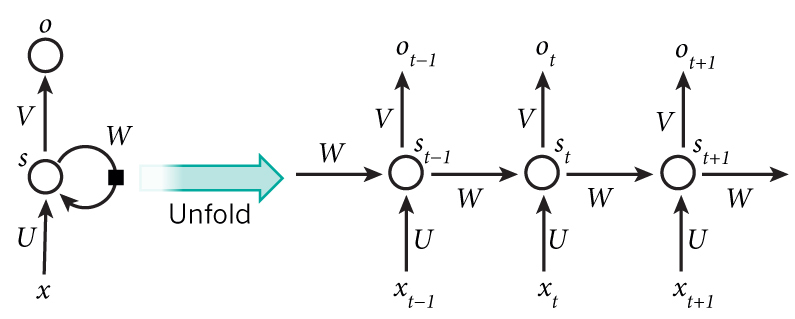
\includegraphics[width=\textwidth]{rnn.jpg}
\caption{Unrolling an RNN unit. Left is the original RNN, right is the unrolled version. $x_t$ is the input at time $t$, $s_t$ is the hidden state of the RNN at time $t$, $o_t$ is the output of the RNN at time $t$. $W$ and $V$ are the weight matrix.}
\caption*{Source: http://www.wildml.com/2015/09/recurrent-neural-networks-tutorial-part-1-introduction-to-rnns/}
\label{fig:unrolled}
\end{figure}

There are three popular types of RNN units, including the vanilla RNN, the LSTM ~\citep{hochreiter1997long}, and the GRU ~\citep{cho2014learning}. The main difference among these three types of RNNs is the choice of the function $f$ in the Equation \ref{eq:rnn}. As shown in Figure \ref{fig:rnn_units}, in the vanilla RNN unit, the $f$ is a simple $tanh$ function. While, in the LSTM and GRU, the $f$ is a combination of several functions. The complex structures inside the LSTM and GRU unit could solve the long-term dependency problems caused by the simple $tanh$ function in the vanilla RNN unit ~\citep{hochreiter1997long}.

\begin{figure}[H]
\centering
\subfloat[Vanilla RNN unit.]{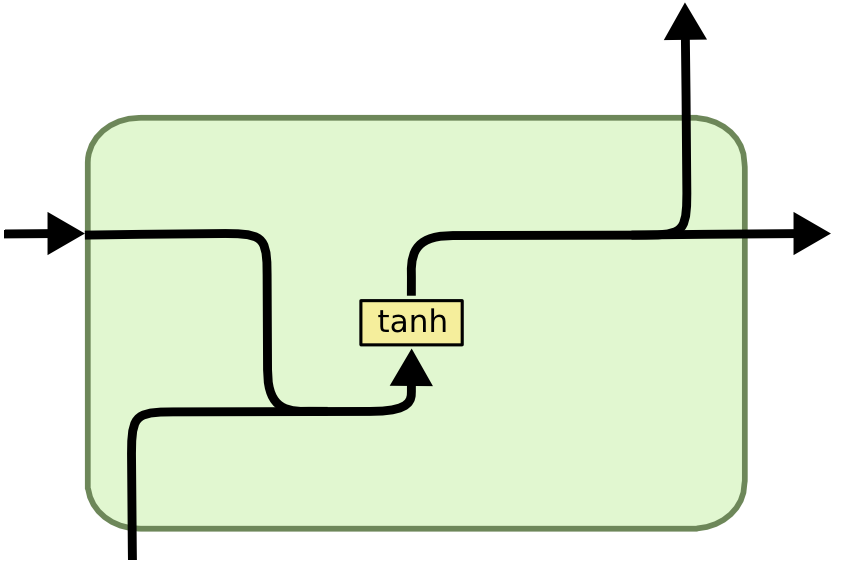
\includegraphics[width=.33\textwidth]{rnn_unit.png}}
\subfloat[LSTM unit.]{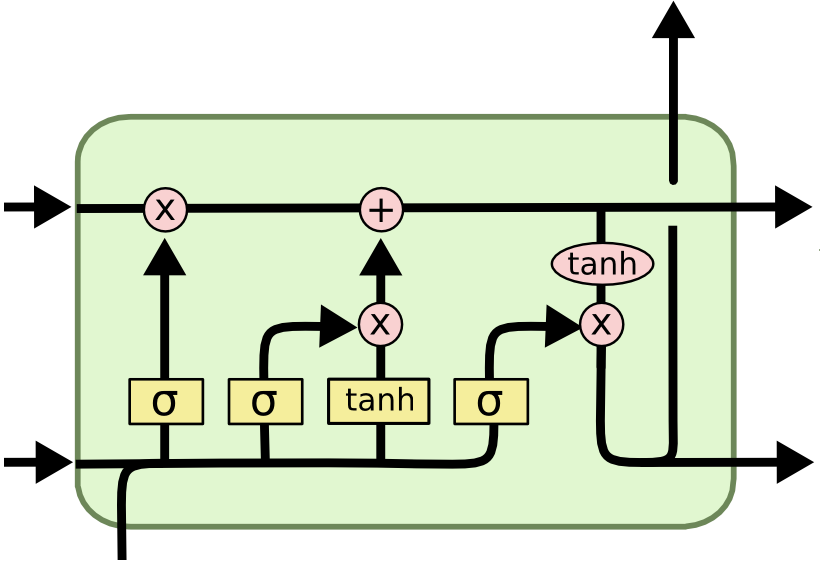
\includegraphics[width=.33\textwidth]{lstm_unit.png}}
\subfloat[GRU unit.]{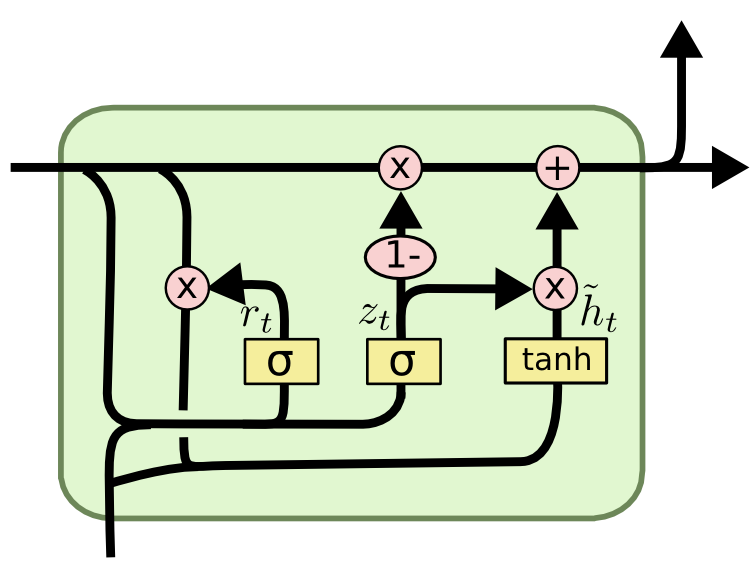
\includegraphics[width=.33\textwidth]{gru_unit.png}}
\caption{Three types of RNN units.}
\caption*{Source: http://colah.github.io/posts/2015-08-Understanding-LSTMs/}
\label{fig:rnn_units}
\end{figure}

Bidirectional RNNs are similar to the 2-layered RNNs, except that the first RNN layer receives the input sequence word by work from left to right, while the second layer gets the input sequence from right to left ~\citep{schuster1997bidirectional}. Therefore, bidirectional RNNs could capture the information before and after the current input data. The RNN unit inside the bidirectional RNNs could be the vanilla RNN unit, the LSTM unit, or the GRU. Figure \ref{fig:birnn} shows a basic bidirectional RNN, we could see that the output $y_t$ is computed based on the concatenation of forward and backward hidden states in the RNN.

\begin{figure}[H]
\centering
\captionsetup{justification=centering,margin=1cm}
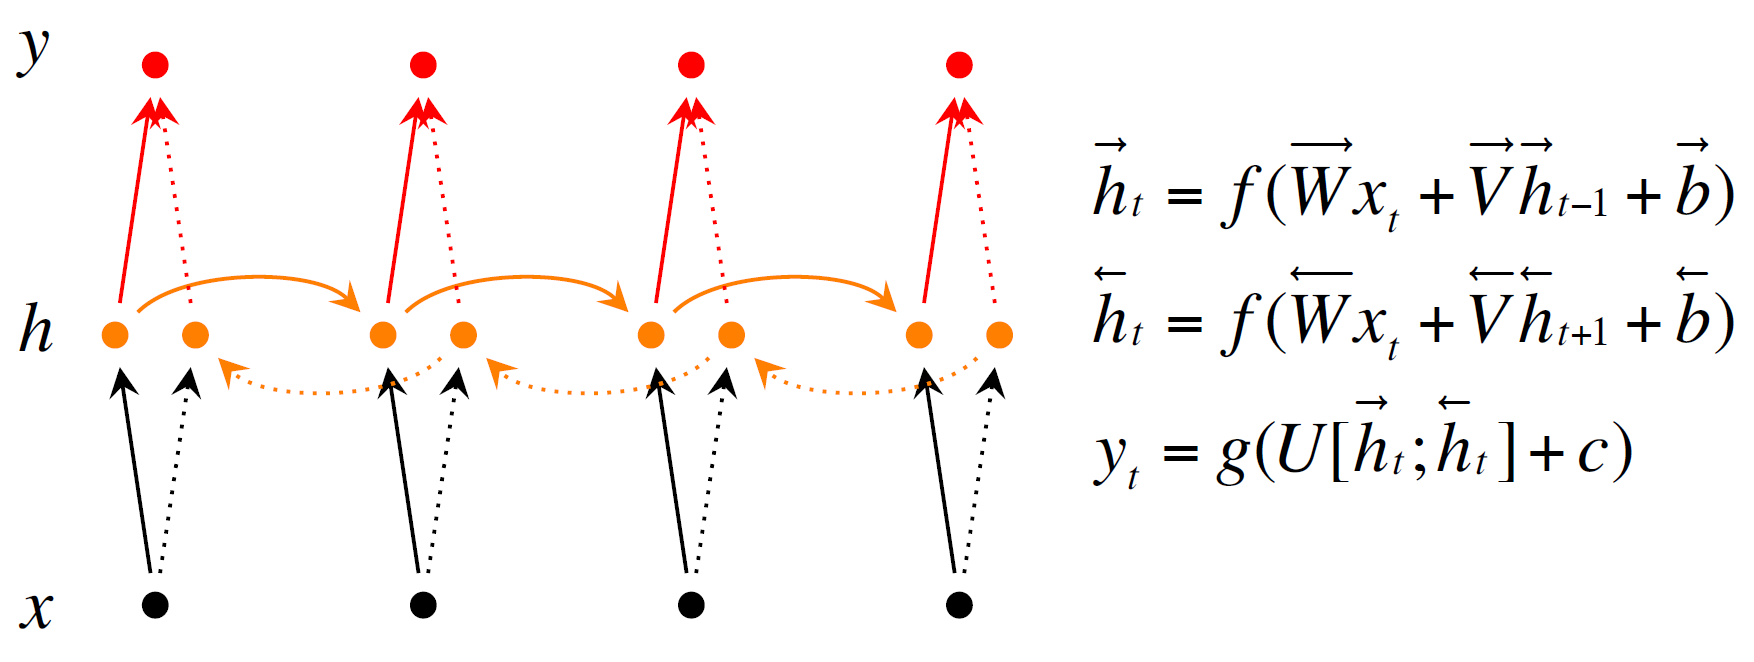
\includegraphics[width=\textwidth]{birnn.png}
\caption{The bidirectional RNN. $\protect\overrightarrow{h_t}$ is the forward RNN hidden state,  $\protect\overleftarrow{h_t}$ is the backward RNN hidden state. $x_t$ is the input at time $t$, $y_t$ is the output at time $t$. $f$ is the function inside the unit, which could be the vanilla RNN, LSTM, and GRU.}
\caption*{Source: http://web.stanford.edu/class/cs224n/lectures/lecture9.pdf}
\label{fig:birnn}
\end{figure}

attention

\subsection{Relevant Literature}
\label{sec:rl_rnn}

\section{Branch Prediction}
\label{sec:bp}

\subsection{Basic Knowledge}
\label{sec:bk_bp}

\subsection{Relevant Literature}
\label{sec:rl_bp}

\section{Dataset}
\label{sec:dataset}
Introduce the branch prediction championship competition and the related dataset.

\section{Training Procedure}
\label{training}
This part introduce the metrics used during training, like dropout, adam optimization, learning rate ...


